\chapter{Results and Discussion}\label{ch:results}
\section{Completeness and interpretation}
All 20 planned graph-by-configuration cells are complete. There are 1000 PDP v2, 1000 Uniform1, 700 Uniform4, and 200 Non-Private final units. The complete sealed U6-A observations provide Spread, Coverage, the CELF denominator, public initialization seed, run identity, and execution provenance for each unit \cite{projectu6}. The deterministic verification for this draft independently recomputed cell statistics and Welch contrasts from those saved scalars, without importing a model or evaluating a graph.

The numerical conclusions below distinguish four kinds of statement. The tables describe observed outcomes. Confidence intervals and the primary test provide inference under the frozen repeat-generation assumptions. Chapter~\ref{ch:method} supplies a conditional privacy theorem. Possible explanations for utility behavior remain hypotheses unless separately identified by controlled evidence. No category is used as a substitute for another.

\section{Coverage across the four configurations}
\begin{table}[htbp]
\centering\small
\caption{Independent confirmation: Coverage mean $\pm$ sample SD (\%). Per graph: Non-Private $n=40$, Uniform1 $n=200$, PDP v2 $n=200$, Uniform4 $n=140$. Source: sealed U6-A saved scalar matrix.}\label{tab:coverage}
\begin{tabular}{lrrrr}
\toprule
Graph & Non-Private & Uniform1 & PDP v2 & Uniform4\\ \midrule
Email & 92.164 $\pm$ 2.273 & 86.005 $\pm$ 12.041 & 86.170 $\pm$ 11.224 & 88.555 $\pm$ 10.945 \\
Bitcoin & 98.689 $\pm$ 0.662 & 88.686 $\pm$ 16.380 & 90.666 $\pm$ 14.489 & 92.074 $\pm$ 10.905 \\
LastFM & 94.961 $\pm$ 1.008 & 80.193 $\pm$ 23.350 & 82.105 $\pm$ 23.332 & 85.315 $\pm$ 20.418 \\
HepPh & 81.653 $\pm$ 5.863 & 72.392 $\pm$ 21.730 & 72.943 $\pm$ 21.225 & 74.484 $\pm$ 21.651 \\
Facebook & 92.608 $\pm$ 2.447 & 79.050 $\pm$ 22.805 & 78.365 $\pm$ 25.009 & 83.621 $\pm$ 18.578 \\
\bottomrule\end{tabular}
\end{table}

Table~\ref{tab:coverage} reports mean and sample SD using every final unit. Non-Private has the highest observed mean on each graph. Uniform4 has a higher observed mean than PDP v2 on each graph. These are properties of the current matrix; they do not establish a universal ordering or make either reference a theoretical upper bound.

The private means conceal wide spreads between runs. Email's PDP mean is 86.170\%, with SD 11.224 pp. The corresponding SDs for LastFM, HepPh, and Facebook are about 23.332, 21.225, and 25.009 pp. Such variation matters when a single trained model is used operationally. A moderate improvement in expected Coverage would not alone ensure reliable utility from one run.

Figure~\ref{fig:distributions} shows the complete empirical Coverage distributions. It uses saved scalars rather than regenerated graph evaluations. The private configurations display broad lower tails on several graphs, whereas Non-Private is more concentrated under the tested repeat protocol. This comparison includes multiple differences in training organization and protection; it is not an isolated estimate of the effect of adding Gaussian noise.

\begin{figure}[htbp]
\centering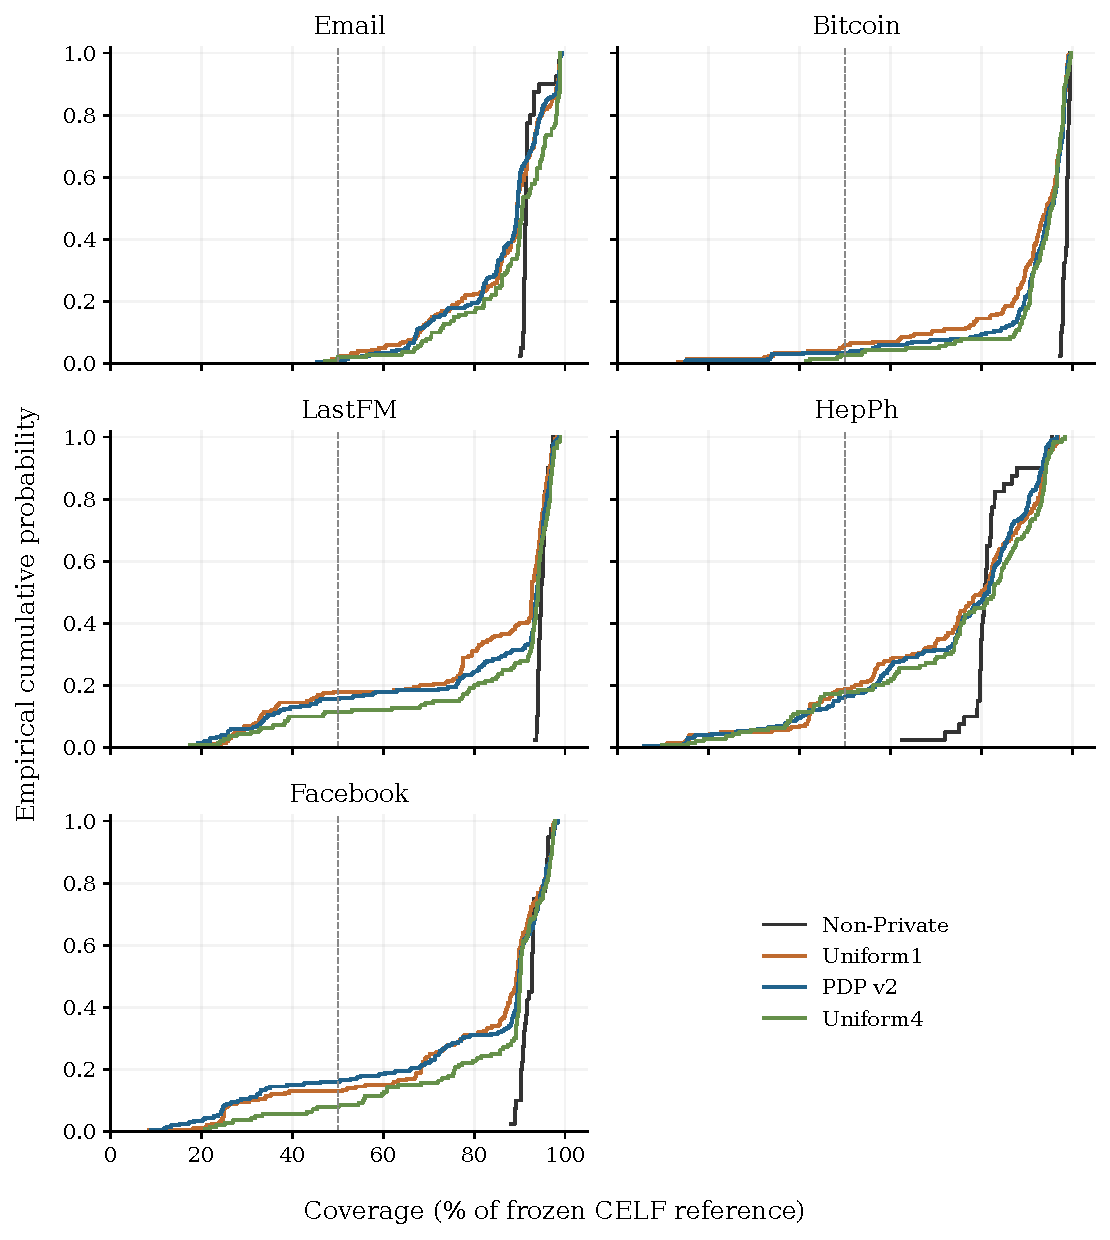
\includegraphics[width=\textwidth]{figures/coverage_distributions.pdf}
\caption{Empirical Coverage distributions from all 2900 final saved scalar outcomes. Each panel is one fixed graph; curves are empirical cumulative distributions. The dashed line marks the strict-low-utility threshold at 50\%. Different reference sample sizes remain as planned.}\label{fig:distributions}
\end{figure}

\section{Primary five-graph comparison}
The main comparison is PDP v2 minus Uniform1, with each graph weighted by one fifth. The verified output is
\begin{align*}
 \widehat D&=+0.7845395873\ \mathrm{pp},\\
 \mathrm{SE}&=0.8839786950\ \mathrm{pp},\qquad \nu=1656.1919278,\\
 p_{\mathrm{one}}&=0.1874667289,\\
 L_{95}&=-0.6702897323\ \mathrm{pp},\\
 \mathrm{CI}_{95}&=[-0.9492939081,\ 2.518373083]\ \mathrm{pp}.
\end{align*}
The frozen one-sided test does not reject at $\alpha=0.05$. The point estimate is positive, but the interval permits a modest negative effect and a positive effect of some size. The evidence therefore does not establish the proposed average utility advantage under the stated protocol.

This conclusion is narrower than saying that personalization is useless. An inconclusive superiority test does not establish equality, and no equivalence margin or equivalence test was approved. Equally, the positive estimate must not be described as a statistically demonstrated improvement. Presenting both the sign and the uncertainty preserves the distinction.

The planning target was 3 pp. The observed estimate is below that target and the reported two-sided 95\% upper endpoint is also below 3. Thus the current approximate interval does not support an improvement of that magnitude; it remains compatible with smaller positive benefits. This comparison concerns the predeclared planning scale, not an externally validated minimum benefit shared by all IM applications.

\section{Graph-specific effects and multiplicity}
\begin{table}[htbp]
\centering\small
\caption{PDP v2 minus Uniform1 (pp). All five primary-gated Holm claims remain closed. 99\% individual intervals form the Bonferroni family; all Welch intervals are approximate. Source: U6-A.}\label{tab:effects}
\begin{tabular}{lrrrr}
\toprule
Graph & Effect & 95\% CI & One-sided $p$ & 99\% CI\\ \midrule
Email & +0.166 & [-2.123, 2.454] & 0.4435 & [-2.847, 3.178] \\
Bitcoin & +1.980 & [-1.060, 5.020] & 0.1006 & [-2.023, 5.982] \\
LastFM & +1.912 & [-2.677, 6.501] & 0.2066 & [-4.129, 7.953] \\
HepPh & +0.551 & [-3.672, 4.773] & 0.3989 & [-5.009, 6.110] \\
Facebook & -0.685 & [-5.390, 4.020] & 0.6126 & [-6.880, 5.509] \\
\bottomrule\end{tabular}
\end{table}

The per-graph effects are positive on Email, Bitcoin, LastFM, and HepPh, and negative on Facebook. Email's effect is only $+0.1655092593$ pp. Bitcoin and LastFM have the largest positive estimates, $+1.979809976$ and $+1.912135540$ pp, respectively. HepPh contributes $+0.5505456634$ pp, while Facebook contributes $-0.6853025024$ pp.

All five ordinary 95\% intervals include zero. More importantly for confirmatory claims, the frozen primary gate is closed, so none of the per-graph Holm claims is established. The raw one-sided values also do not cross 0.05. Choosing Bitcoin or LastFM after observing the matrix would not produce a successful replacement for the predeclared five-graph research question.

Figure~\ref{fig:effects} displays the graph-specific intervals together with the primary estimate. It separates the uncertainty of each graph effect from the uncertainty of the fixed average. The average interval is narrower because the estimator combines independent arm estimates, not because the five graphs are treated as a large IID graph sample.

\begin{figure}[htbp]
\centering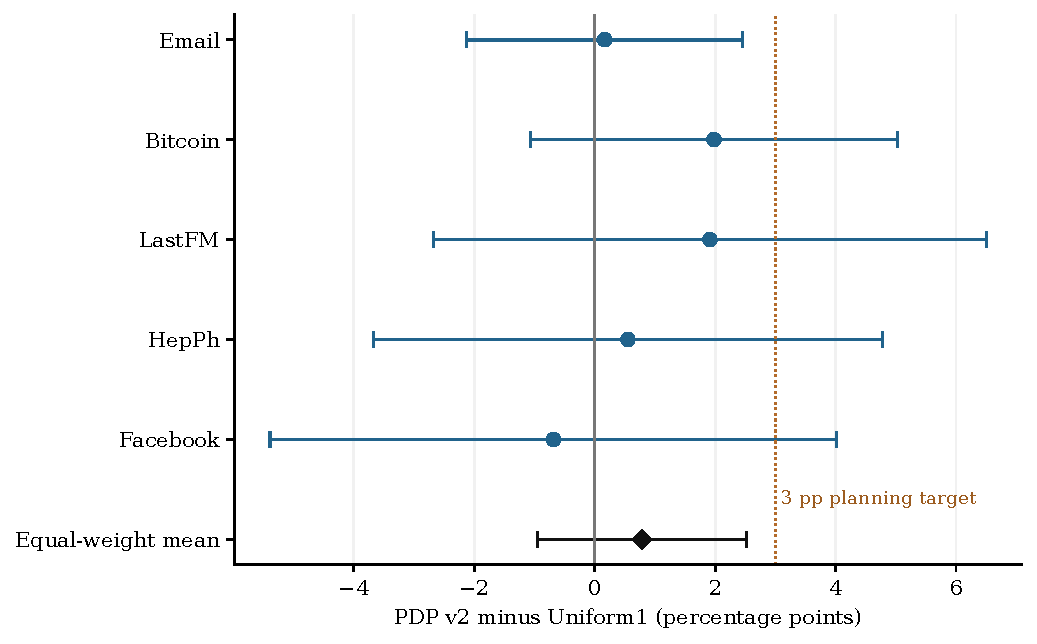
\includegraphics[width=.92\textwidth]{figures/primary_effects.pdf}
\caption{PDP v2 minus strict Uniform1, in percentage points. Bars are individual approximate two-sided 95\% Welch intervals. The bottom point is the fixed equal-weight five-graph estimate; per-graph intervals are not multiplicity-adjusted here. Sources: U6-A saved observations and frozen analysis.}\label{fig:effects}
\end{figure}

\section{Gaps to relaxed privacy and Non-Private references}
\begin{table}[htbp]
\centering\small
\caption{PDP v2 minus the relaxed Uniform4 and Non-Private references (pp), with individual approximate 95\% intervals. These are secondary estimations, not alternative primary success tests. Source: U6-A.}\label{tab:references}
\begin{tabular}{lrrrr}
\toprule
Graph & vs Uniform4 & 95\% CI & vs Non-Private & 95\% CI\\ \midrule
Email & -2.385 & [-4.783, 0.014] & -5.994 & [-7.711, -4.278] \\
Bitcoin & -1.408 & [-4.119, 1.303] & -8.023 & [-10.054, -5.993] \\
LastFM & -3.210 & [-7.907, 1.487] & -12.855 & [-16.124, -9.587] \\
HepPh & -1.541 & [-6.199, 3.117] & -8.710 & [-12.187, -5.233] \\
Facebook & -5.257 & [-9.908, -0.605] & -14.243 & [-17.811, -10.675] \\
\bottomrule\end{tabular}
\end{table}

Against Uniform4, the fixed five-graph average difference is $-2.760097453$ pp, with two-sided 95\% interval $[-4.526931435,-0.9932634706]$ pp. This secondary estimate describes a utility deficit relative to the specified relaxed mechanism. It is consistent with an average gap under the repeat model, but is not a substitute primary success test or proof that Uniform4 dominates all other mechanisms.

Facebook has the largest observed PDP--Uniform4 deficit, $-5.256527445$ pp. The other four deficits range from about $-1.408$ to $-3.210$ pp. Their individual intervals vary, and several include zero. Uniform4's own low tails show that a smaller Gaussian scale does not eliminate variability in this training system.

Against Non-Private, the equal-weight average difference is $-9.965100134$ pp, with interval $[-11.26440434,-8.66579593]$ pp. Per-graph estimates range from about $-5.994$ pp on Email to $-14.243$ pp on Facebook. These gaps quantify the difference between the complete private and ordinary training routes, not the isolated cost of a single privacy operation.

Uniform4 does not carry the original heterogeneous target 1/2 compliance guarantee. Non-Private carries no protection. Neither is a fair same-policy replacement for PDP v2 merely because its mean is higher. The result instead identifies how far the current personalized mechanism lies below two differently constrained reference procedures.

\section{Severe low utility and observed variability}
\begin{table}[htbp]
\centering\small
\caption{Full-range and severe-low-utility results. Coverage and cellwise 95\% Clopper--Pearson intervals are percentages. Intervals concern each cell under the IID repeat model, without simultaneous adjustment. Source: U6-A.}\label{tab:low}
\begin{tabular}{llrrrr}
\toprule
Graph & Method & Min--max & $<50\%$ & Rate (\%) & CP interval (\%)\\ \midrule
Email & Non-Private & 90.046--98.843 & 0/40 & 0.00 & [0.00, 8.81] \\
Email & Uniform $\epsilon=1$ & 45.602--98.843 & 3/200 & 1.50 & [0.31, 4.32] \\
Email & PDP v2 & 45.370--99.306 & 1/200 & 0.50 & [0.01, 2.75] \\
Email & Uniform $\epsilon=4$ & 47.222--98.843 & 2/140 & 1.43 & [0.17, 5.07] \\
Bitcoin & Non-Private & 97.328--99.525 & 0/40 & 0.00 & [0.00, 8.81] \\
Bitcoin & Uniform $\epsilon=1$ & 13.242--99.703 & 12/200 & 6.00 & [3.14, 10.25] \\
Bitcoin & PDP v2 & 14.727--99.644 & 7/200 & 3.50 & [1.42, 7.08] \\
Bitcoin & Uniform $\epsilon=4$ & 41.330--99.703 & 4/140 & 2.86 & [0.78, 7.15] \\
LastFM & Non-Private & 93.459--97.242 & 0/40 & 0.00 & [0.00, 8.81] \\
LastFM & Uniform $\epsilon=1$ & 19.543--98.188 & 36/200 & 18.00 & [12.94, 24.04] \\
LastFM & PDP v2 & 19.070--98.582 & 31/200 & 15.50 & [10.78, 21.27] \\
LastFM & Uniform $\epsilon=4$ & 17.494--98.976 & 16/140 & 11.43 & [6.68, 17.90] \\
HepPh & Non-Private & 62.608--95.462 & 0/40 & 0.00 & [0.00, 8.81] \\
HepPh & Uniform $\epsilon=1$ & 9.707--96.898 & 38/200 & 19.00 & [13.81, 25.13] \\
HepPh & PDP v2 & 5.744--96.611 & 32/200 & 16.00 & [11.21, 21.83] \\
HepPh & Uniform $\epsilon=4$ & 9.765--98.449 & 25/140 & 17.86 & [11.90, 25.22] \\
Facebook & Non-Private & 88.122--97.751 & 0/40 & 0.00 & [0.00, 8.81] \\
Facebook & Uniform $\epsilon=1$ & 8.362--97.719 & 26/200 & 13.00 & [8.67, 18.47] \\
Facebook & PDP v2 & 8.806--98.480 & 32/200 & 16.00 & [11.21, 21.83] \\
Facebook & Uniform $\epsilon=4$ & 20.684--97.719 & 11/140 & 7.86 & [3.99, 13.62] \\
\bottomrule\end{tabular}
\end{table}

Table~\ref{tab:low} preserves every extreme value and all strict-low-utility events. PDP v2 has 103 of 1000 outcomes below 50\%; Uniform1 has 115 of 1000; Uniform4 has 58 of 700; and Non-Private has zero of 200. These are whole-matrix inventory totals. They should not be assigned a pooled binomial confidence interval as if the five heterogeneous graph distributions were identical.

Within graphs, PDP's event counts are 1/200, 7/200, 31/200, 32/200, and 32/200 in the stated graph order. Uniform1 has 3/200, 12/200, 36/200, 38/200, and 26/200. PDP therefore has fewer observed events on the first four graphs but more on Facebook. This mixed pattern does not justify a general stability-superiority claim, and the frozen analysis does not supply a separate confirmatory risk-success test.

Clopper--Pearson intervals quantify the cellwise event-rate uncertainty under the IID model. They are individual intervals, not a joint guarantee across all 20 cells. The saved Hoeffding alternatives offer conservative references if only independence and boundedness are used. No interval procedure converts a low observed count into a policy-independent guarantee against a poor future model.

The minima are consequential. PDP reaches 5.744\% on HepPh and 8.806\% on Facebook; Uniform1 reaches 9.707\% and 8.362\% on those graphs. These outcomes remain in every mean and SD. They were not treated as errors solely because they were poor. Conversely, different sample sizes make simple minimum-based rankings of methods unfair: a method run 200 times has more opportunities to exhibit an extreme than one run 40 times.

PDP has a smaller observed sample SD than Uniform1 on four graphs, but not Facebook. LastFM's SD difference is very small. These descriptive comparisons do not establish lower population variance, stochastic dominance, or a significant severe-loss reduction. Practical use would require an independently justified risk criterion as well as a mean objective.

\section{Sensitivity analyses and inference limits}
The predeclared, saved bootstrap percentile interval is $[-0.9025217677,2.533756590]$ pp, based on 10,000 within-cell resamples with analysis seed 20261104. It is close to the primary Welch interval in this record and also includes zero. It remains a sensitivity analysis dependent on the within-cell sampling model, not an independently randomized second experiment.

The saved distribution-free Hoeffding interval, in percentage points, is much wider:
\[[-28.19371919,\ 29.76279837].\] Its width follows from conservative public Coverage ranges rather than the observed variances. It illustrates the cost of weaker distributional assumptions. Selecting whichever interval happens to support a desired conclusion would defeat the frozen plan.

The primary inference conditions on the approved generation model, valid provenance, and recovery treatment. Scalar verification establishes arithmetic agreement and saved-data consistency; it cannot certify ideal IID randomness, rule out every source fault, or prove privacy. The inferential statements should therefore retain their approximate and conditional character.

\section{Development versus confirmation}
The final four-configuration development matrix gave a five-graph average PDP--Uniform1 difference of approximately $-1.100$ pp. Graph-specific development differences were $+4.630$, $+8.373$, $-0.725$, $-3.573$, and $-14.203$ pp. Independent confirmation instead gives $+0.785$ pp on average with a different sign pattern. No algorithmic change is inferred from that difference; small development cells and fresh initialization and secret trajectories can produce different estimates.

The development matrix had only five observations per cell. Its SDs were useful planning proxies but uncertain descriptions of the repeat distribution. In particular, Facebook's large negative development contrast should not be discarded, and the later smaller negative confirmation estimate should not be presented as correction of an invalid old result. Both are valid observations at their respective stages.

The development effect signs and ranks are insufficient to select a globally favorable initialization subset. Public seeds do not encode a shared secret path across methods. Removing a seed after seeing outcomes changes the analysis population and can create a misleading story. The complete 100-row development evidence is retained separately in Appendix~\ref{app:development}; none enters the 2900-unit confirmation estimate.

\section{Gaussian-path diagnostics and historical candidates}
A historical controlled G2 investigation varied Gaussian trajectories while holding the specified initialization and outer retained-graph witness fixed. For one LastFM setting, Coverage changed from approximately 96.848\% to 50.118\%, a difference of $-46.730$ pp. A Facebook setting changed from about 72.632\% to 93.031\%, or $+20.399$ pp. The saved control witnesses support the observation that Gaussian training paths can materially alter final rankings and Coverage.

This diagnostic does not allocate all observed variance among initialization, outer sampling, Gaussian innovations, graph structure, and their interactions. It contains a small controlled set rather than an exhaustive factorial study. It also concerns historical development mechanisms and should not be presented as a new randomized ablation of the 2900 final runs.

G3 parameter averaging and C3 row-sum stability exploration were not accepted by their frozen development screens. C3 completed all 100 outcomes and still failed the required per-graph gates, even though some graph averages improved. These failures matter because a cross-graph average can mask local regressions. They remain historical evidence, not additional confirmed versions of PDP v2.

New Matched PDP froze 2307 coordinates and privately trained a 33-coordinate head. In its five-run-per-graph development record, it had higher mean Coverage than full-training PDP v2 on four graphs, but was about 2.114 pp lower on HepPh. Its SD was smaller on all five graphs, and it had zero severe-low-utility events in 25 runs. These observations are not hidden simply because they challenge the usefulness of full private training.

The frozen-backbone comparison matches a conditional ideal privacy-bound framework, not exact privacy loss or a single causal factor. It changes trainable dimension, gradient geometry, and representation learning while using independent secret trajectories. Its results motivate research into training-space choices, but do not establish that a random frozen backbone is always sufficient or that head-only training is the final superior mechanism.

\section{Budget utilization and possible utility explanations}
The mechanism uses personalization in a concrete way: strict identities have lower participation and the base noise scale is 260 rather than 486. It is therefore incorrect to say that no heterogeneous allowance is used. Nevertheless, targets 2 and 4 both have $p_v=1$ and the same approximately 1.982 base bound, leaving no further response to the budget-4 label.

There is a plausible signal--noise tradeoff. Reduced Gaussian noise can benefit optimization, while removing strict nodes and incident edges can alter slot topology, subgraph content, and useful gradients. Double clipping can further change signal direction and magnitude. The current experiment compares the complete mechanisms, so it cannot quantify the contribution of each component or prove that one exactly cancels another.

The full-coordinate noise geometry offers another hypothesis. At the PDP learning-rate and denominator, each unprojected coordinate has one-update Gaussian SD $0.005\cdot260/16=0.08125$. This does not become small merely because only 32 coordinates are projected. Noise enters hidden-layer and attention parameters too, and a nonlinear score ordering can change sharply near ties. Parameter-space noise energy is calculable, but its mapping to the observed Coverage tail is not a proven causal decomposition.

The scientifically supported explanation is therefore a limit on current evidence: the frozen mechanism did not demonstrate a reliable average advantage, and severe variability persisted. The findings are compatible with multiple mechanism-level hypotheses. A future study would need new authorization, a justified design, and frozen hypotheses to separate them.

\section{Scientific implications and threats to validity}
The study separates three propositions that are sometimes conflated: heterogeneous caps can be met by the stated ideal mechanism; lower base noise can be permitted by personalization; and a reliable utility improvement is empirically obtained. The first two have conditional mathematical support. The third is not established by this confirmation matrix.

Internal validity depends on the source and execution lineage, graph isolation, fixed ranking rules, and approved continuation decisions. Construct validity is limited by one-step Coverage relative to CELF rather than actual social outcomes. Statistical validity depends on the repeat-generation assumptions and approximate inference, with low-tail intervals and sensitivity analyses providing context. External validity is restricted to five prepared graphs, one split, one architecture, one policy mixture, and one budget allocation.

Finally, publication privacy is a separate threat boundary. Raw scalar evaluations and model collections may reveal information not protected by the single-model theorem. This dissertation draft is prepared for researcher and supervisor review; its existence does not authorize a general public release of the underlying restricted artifacts. Future claims should retain these limits even if a later mechanism produces a significant utility gain.
